\section{Spectroscopy}
\label{sec:spectroscopy}

The Light of Knowledge is a common expression, but it fits especially in the
spectroscopy context. Spectroscopy is the broad field of study that measures
and interprets the interaction between matter and electromagnetic radiation
as a function of wavelength or frequency. Most of our knowledge regarding atoms and molecules 
comes from examining their interactions with electromagnetic radiation; 
as a result, various parts of the electromagnetic spectrum supply
different types of information (see Figure \ref{fig:EM_spectrum}). The
molecular transitions, such as rotational, vibrational and electronic excitation, 
are characterized via interactions in different regions of the electromagnetic
spectrum, as shown in Table \ref{tab:electromagnetic_spectrum}. Spectroscopic
characteristics are like molecular fingerprints.

\begin{figure}[!htb]
    \centering
    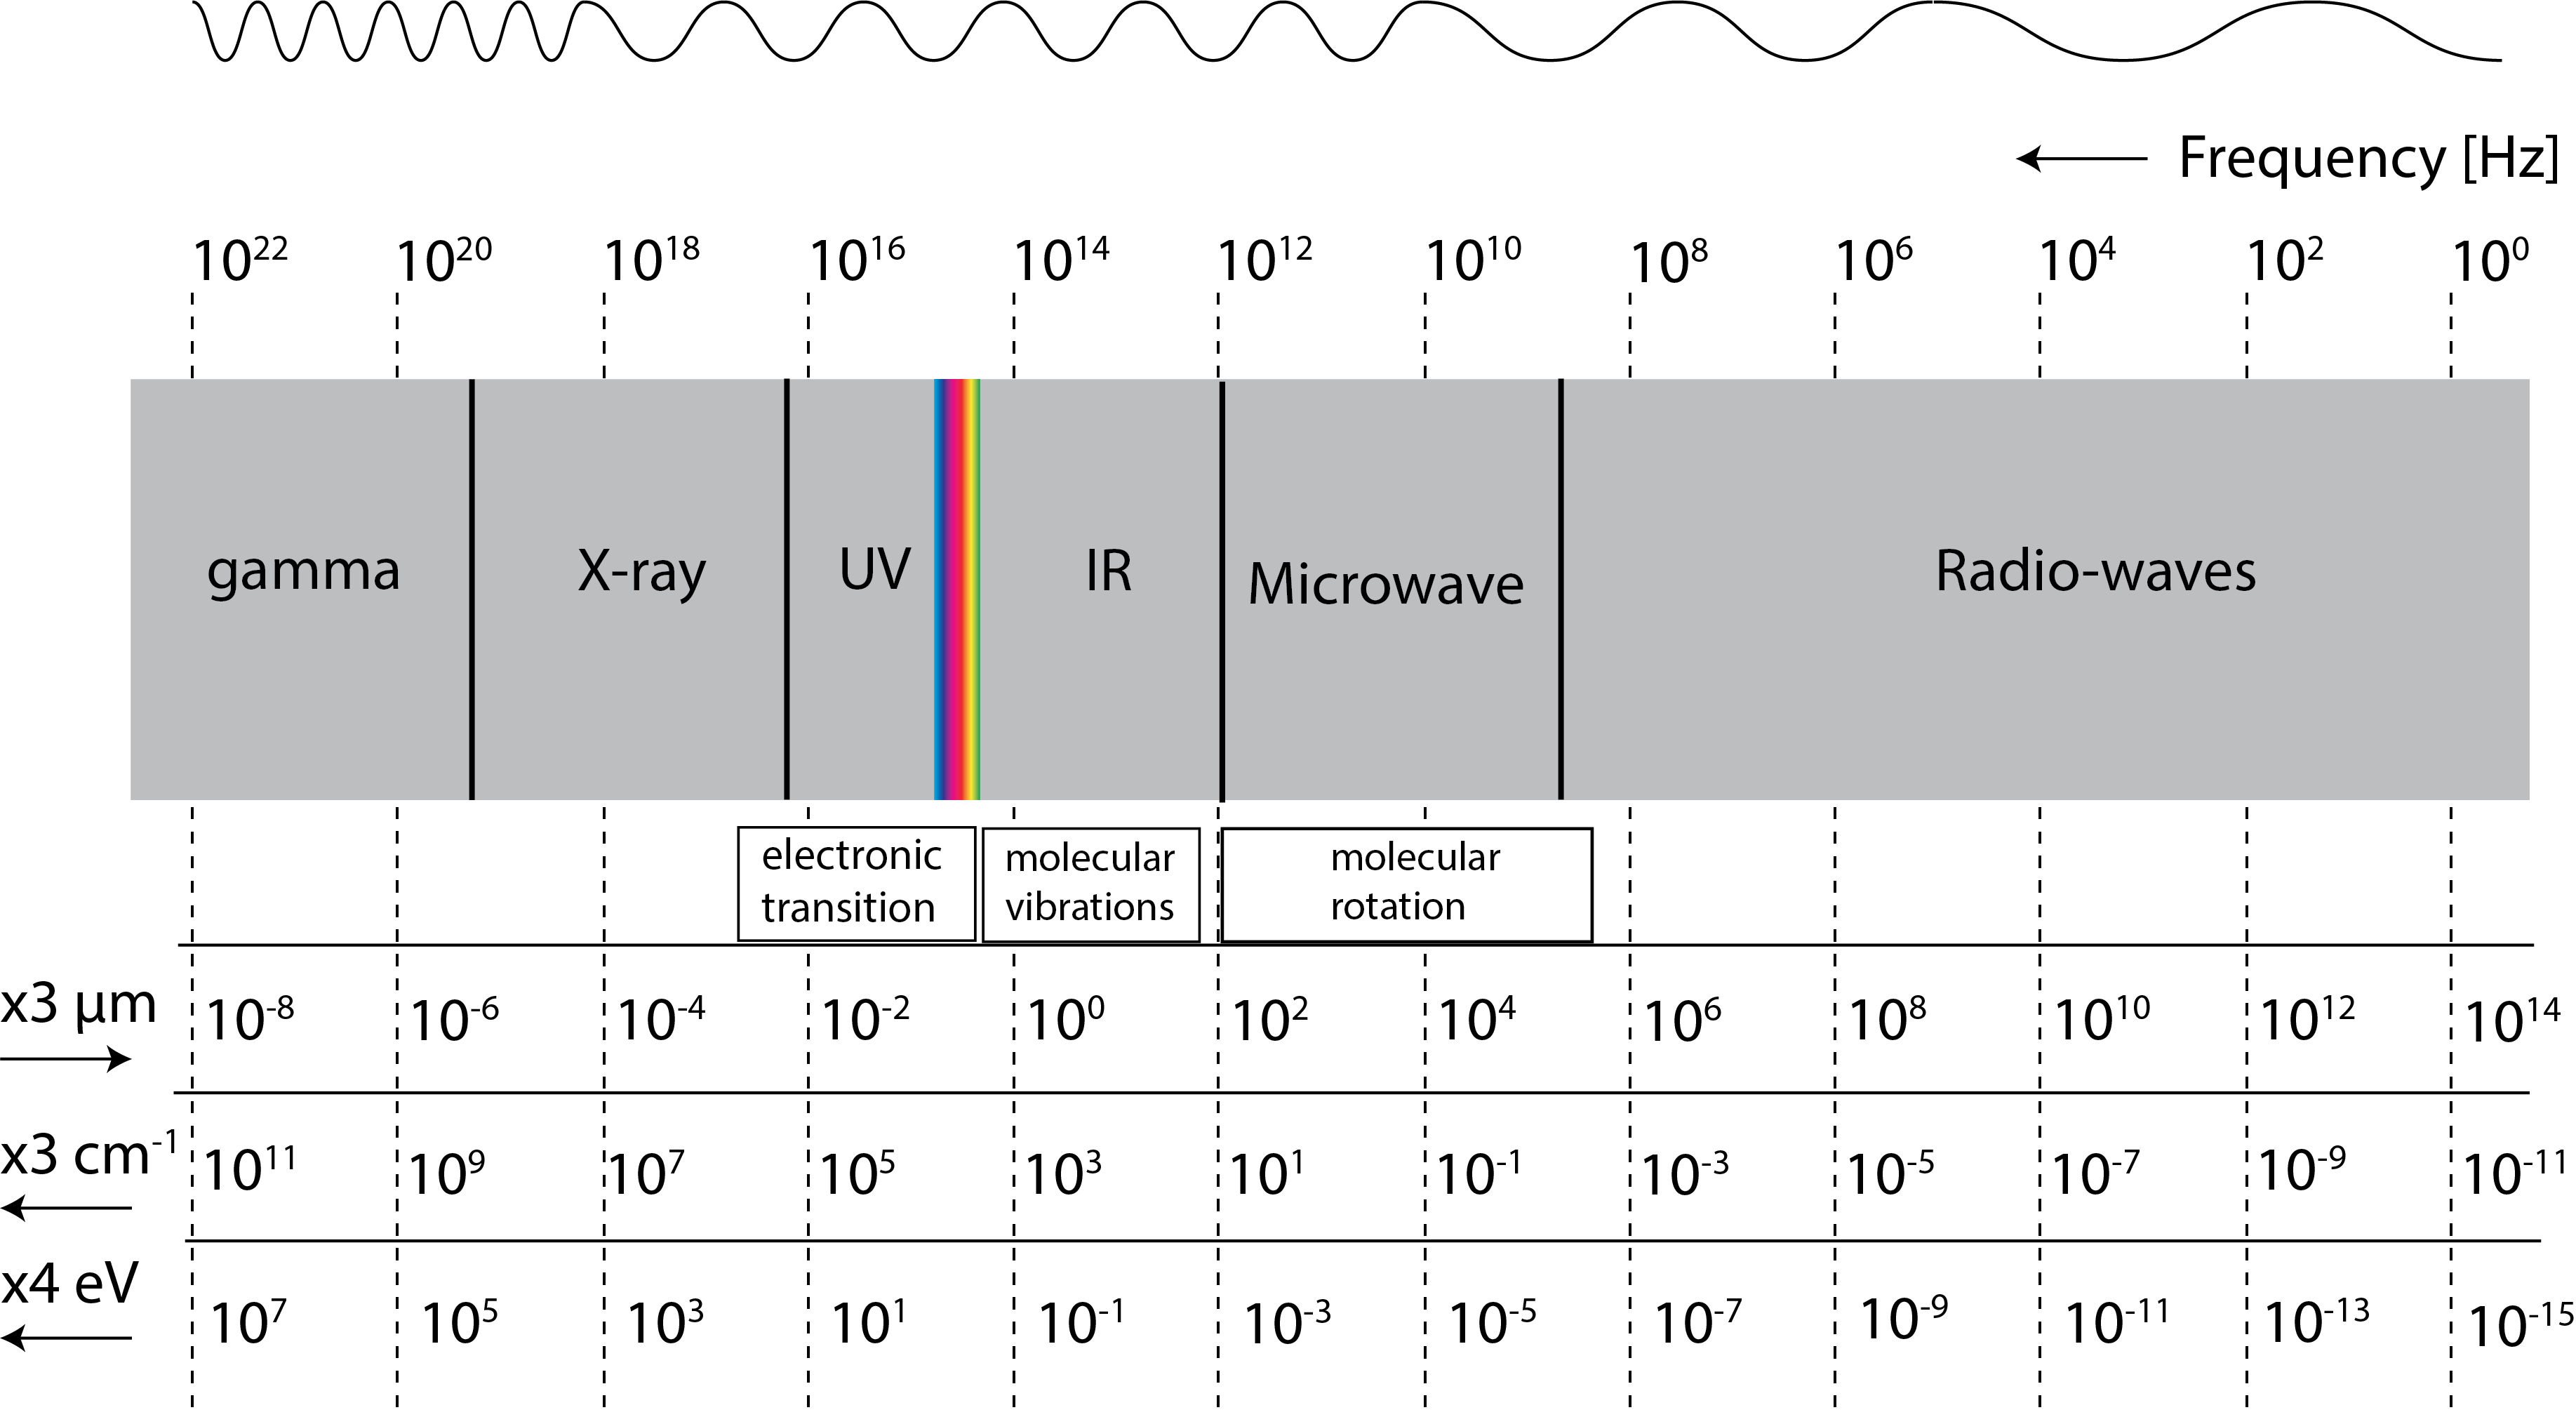
\includegraphics[width=0.9\textwidth]{figures/intro/EM_spectrum_1.png}
    \caption{Schematic diagram of the electromagnetic spectrum, the rainbow-coloured inset shows the visible spectrum. The vertical dashed line indicates a corresponding comparison to the different unit systems as labeled on the left, and \qt{x3} and \qt{x4} indicate that the scale value is multiplied by factors 3 and 4, respectively.}
    \label{fig:EM_spectrum}
\end{figure}

\begin{table}[!htb]
    \centering
    \caption{Dominant types of molecular transitions in each region of the electromagnetic spectrum}
    \begin{tabular}{lccc}
        \toprule
        \multicolumn{2}{c}{\textbf{Region of Spectrum}} & \textbf{Energy [cm$^{-1}$]} & \textbf{Molecular transitions} \\\midrule
        \multicolumn{2}{c}{\emph{Ultraviolet (UV)}} && \multirow{4}*{Electronic}\\
        & far & $10^6 - 50,000$ & \\
        & near & $50,000 - 26,300$ & \\
        \addlinespace
        \multicolumn{2}{c}{\emph{Visible (Vis)}} & $26,300 - 12,800$ & \\
        \midrule\addlinespace
        \multicolumn{2}{c}{\emph{Infrared (IR)}} && \multirow{4}*{Vibrational} \\
        & near & $12,800 - 4000$ & \\
        & mid  & $4000 - 200$ & \\
        & far  & $200 - 10$ & \\
        \midrule\addlinespace
        \multicolumn{2}{c}{\emph{Microwave (THz)}} & $10 - 0.01$ & Rotational \\
        \bottomrule\hline\\
    \end{tabular}
    \label{tab:electromagnetic_spectrum}
\end{table}


Spectrochemical analysis was invented in 1860 by
\citet{kirchhoff_chemical_1860}, but it saw limited use until the 1930s. Since
the discovery of the first molecules in space by their optical spectra, i.e.,
CN and CH \cite{dunham_jr_interstellar_1937, adams_quoted_1937,
    mckellar_evidence_1940, mckellar_wave_1940}, spectroscopy has been successfully
used in astronomy to identify new molecular species and determine physical and
chemical conditions such as gas excitation temperatures and chemical
abundances. Over the past two decades, spectral data has significantly increased from astronomical observations ranging from the UV-vis to the $mm$ and $cm$ wavelength region. A direct comparison with astronomical data is made possible
by laboratory spectroscopic investigations of gas-phase molecules, which has
significantly aided the interpretation of astrophysical findings (see Figure
\ref{fig:astrochemistry-flow-chart}).

\begin{figure}[!htb]
    \centering
    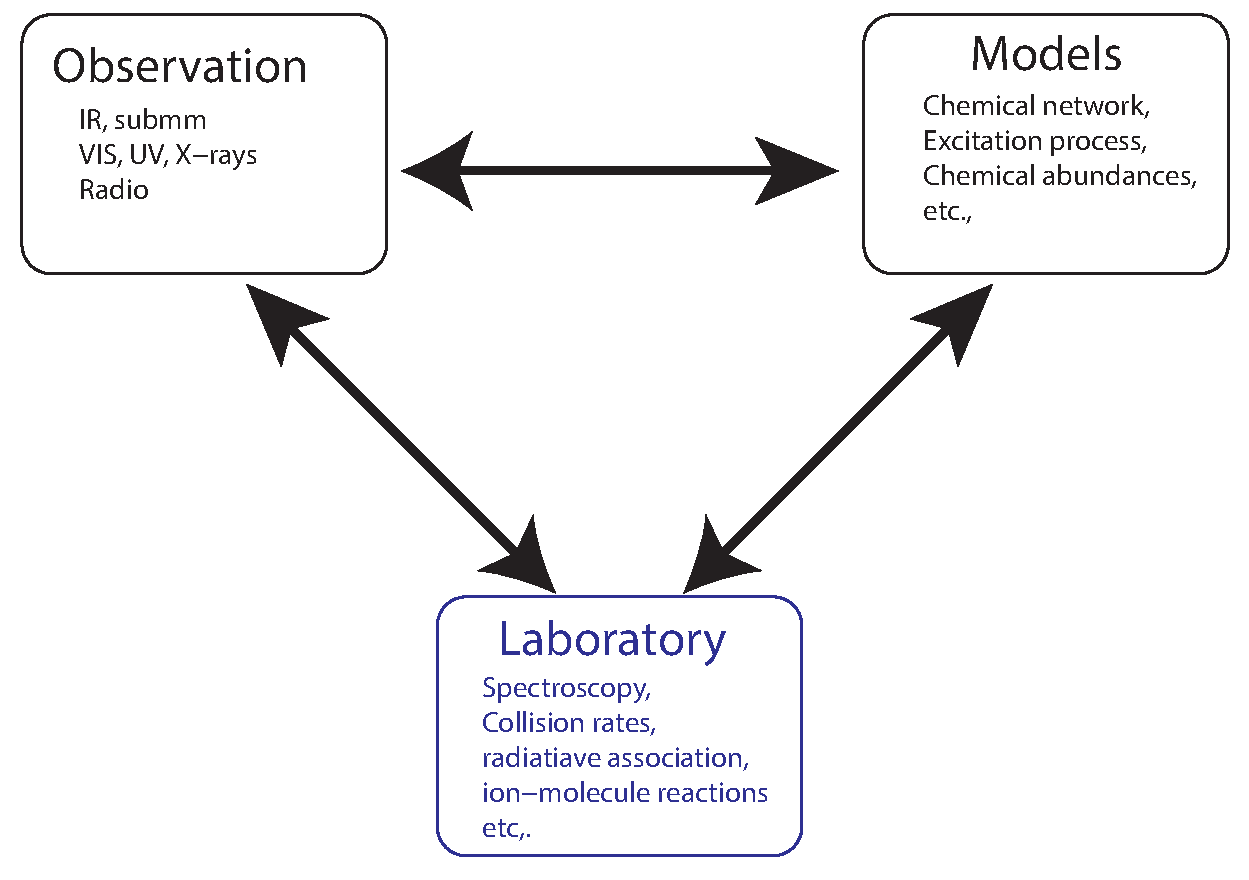
\includegraphics[width=0.8\textwidth]{figures/intro/astrochemistry-flow-chart.pdf}

    \caption{The triangular approach of observations, models, and laboratory studies is necessary to address astrochemistry questions. Examples for every category are provided in smaller fonts with respective boxes. \enquote{Laboratory} implies both experimental and theoretical work. The blue coloured box indicates the area focused on in this thesis.}
    \label{fig:astrochemistry-flow-chart}

\end{figure}

\subsubsection*{Absorption Spectroscopy}

Traditionally spectroscopic measurements of vibrational and rotational
transitions for molecules are recorded via direct absorption techniques to
detect radiation absorption as a function of frequency or wavelength due to its
interaction with the molecule sample. Since all of the atoms and molecules have
distinct and distinguishable energy levels, a measurement of the absorption
lines from incident radiation permits the identification of the absorbing
species. The absorption spectrum is the change in absorption intensity as a
function of frequency (see Figure \ref{fig:absorption_spectroscopy}).\\

\begin{figure}[!htb]
    \centering
    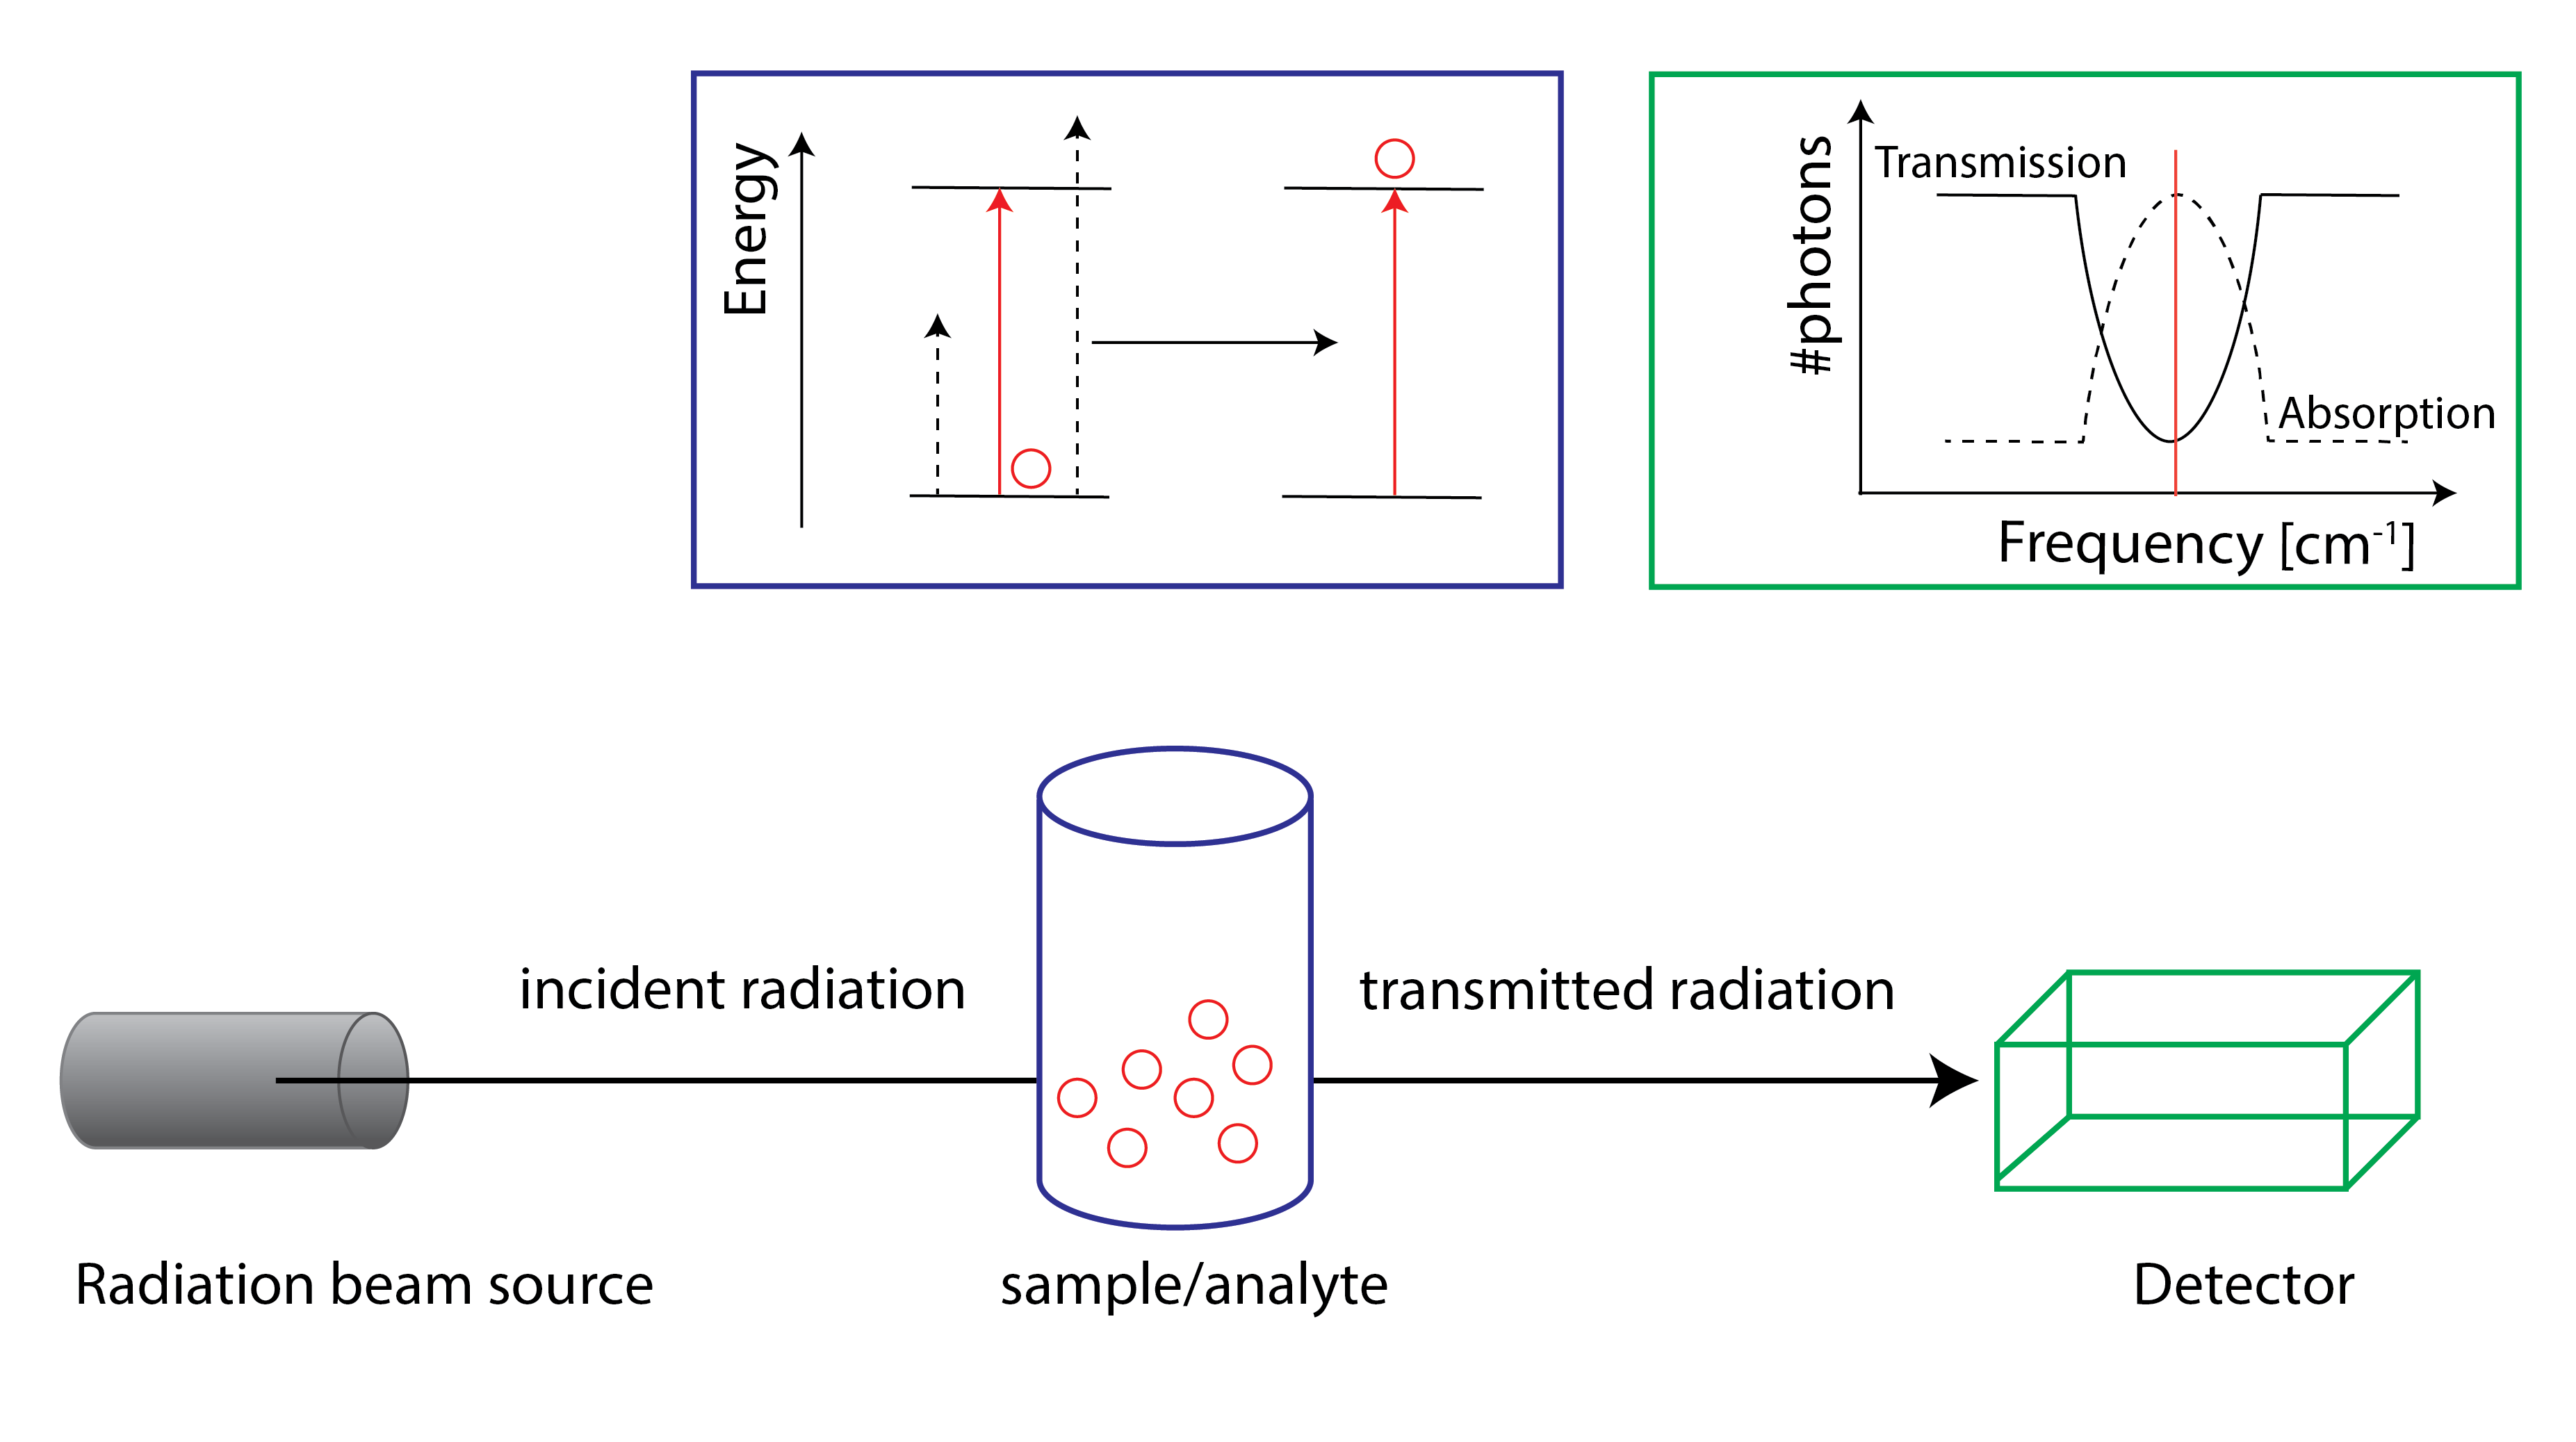
\includegraphics[width=0.8\textwidth]{figures/intro/Absorption.png}
    \caption{Schematic diagram to describe the principle of absorption spectroscopy.}
    \label{fig:absorption_spectroscopy}
\end{figure}

However, these conventional absorption techniques are very challenging to
record spectra of gas-phase molecular ions, especially of highly reactive,
open-shell species, since it is difficult to produce them in sufficient
number density. Another complication arises from background contamination from
other species during the formation process. Oka's \cite{oka_taming_2015} search
for the infrared spectrum of CH$_5^+$ using a discharge through a
CH$_4-$H$_2-$He mixture is a well-known illustration of this challenge.

\subsubsection*{Fourier-Transform Spectroscopy}
Fourier-transform spectroscopy (FTS) is a technique used in the field of spectroscopy to obtain a high-resolution spectrum of molecules. 
This technique is conceptually different from direct absorption spectroscopy.
The FTS is based on the Fourier transform of a time-domain signal, which is obtained by 
measuring the intensity of light emitted or absorbed by the molecules as a function of time.
The FTS technique using microwave radiation is a well-known powerful tool for the study of rotational transitions of molecules, known as Fourier Transform MicroWave (FTMW) spectroscopy. In FTMW, microwave pulse radiation excites a molecule's rotational energy levels and is subsequently probed with a high-resolution Fourier transform spectrometer, which detects the microwave radiation emitted from the molecule as it relaxes to its original state (free induction decay). 
Pate group at the University of Virginia has developed a broadband Chirped-Pulse Fourier Transform MicroWave \text{(CP-FTMW)} spectrometer, which is capable of recording spectra with $>1000$-fold improvement in the rate at which the data can be acquired \cite{brown_rotational_2006, brown_broadband_2008, park_perspective_2016}.

However, these techniques are not necessarily available for smaller molecular ions due to 
very high frequencies of the rotational transitions ($100-500 $ GHz in our study).
Therefore, another form of spectroscopy, known as action spectroscopy, is employed in this thesis study to record both the rotational and vibrational spectra of molecular ions.

\subsubsection*{Action Spectroscopy}

In action spectroscopy techniques, using sensitive mass spectrometry, a change in the chemical composition of ions is monitored when they interact with resonant radiation light instead of the absorption of photons by molecular ions.
\citet{asvany_understanding_2005} successfully employed one such technique in a
cryogenic ion trap to record the infrared spectrum of the elusive CH$_5^+$
molecular ion (see Section \ref{subsec:action:methods:vibrational:LIR} and
\ref{subsec:action:methods:vibrational:LIICG}).

Action spectroscopy can offer several advantages, such as mass selection and
storage in a cold ion trap, leading to uncontaminated spectra and narrow line
widths. In the next section, we shall discuss the cryogenic ion trap techniques
to isolate and confine molecular ions before continuing to describe action spectroscopy
techniques in more detail for vibrational and rotational transitions of molecular ions.
